%--------------------------------------------------------------------------
\chapter{APPLICATIONS AND CONCLUSION}

%TODO: add tests to confirm results

%--------------------------------------------------------------------------
\section{Single and multi-threaded command line tools}

This section exemplifies the use of the framework developed in the previous chapter by defining two command line tools for computing combination matrices of self-derivation. The first of them computes all solutions for a given row and problem size using a single thread of execution, while the second utilizes several threads. The single-threaded application is reasonably fast for small row and problem sizes. As input sizes grow, the number of solutions grows dramatically, and a single thread of excution becomes insufficient.

%--------------------------------------------------------------------------
\begin{lstlisting}[caption={A single-threaded command line tool.},label={singleMain}]
int main(int argc, char *argv[]) {
    if (argc < 3) {
        printf("Enter a problem size and a row!\n");
        return -1;
    }

    common_data commonData;
    createCommonData(&commonData, argc, argv);

    thread_data data;
    createThreadData(&data, &commonData);

    clock_t start = clock();
    writeSolutions(&data, &commonData, 0, commonData.numTops);

    printf("%f seconds elapsed.\n", ((double) (clock() - start)) / CLOCKS_PER_SEC);
    printf("%lu solutions found!\n", data.counter);

    destroyThreadData(&data);
    destroyCommonData(&commonData);

    return 0;
}
\end{lstlisting}

\begin{enumerate}
\item The inputs are the standard command line inputs, that is, the number of arguments, and the array of strings containing them.
\item Line 2 checks that at least three arguments were passed and, if not, line 3 prints usage instructions to the console and line 4 returns an error.
\addtocounter{enumi}{4}
\item Line 7 creates an empty thread-common data structure and line 8 calls Listing~\ref{createCommonData} to fill it.
\addtocounter{enumi}{2}
\item Line 10 creates an empty thread-specific data structure and line 11 calls Listing~\ref{createThreadData} to fill it.
\addtocounter{enumi}{2}
\item Line 13 computes the current time and stores it in a variable. Line 14 calls Listing~\ref{writeSolutions} to write solutions for all tops to a single text file.
\addtocounter{enumi}{2}
\item Line 16 computes the time after the call to Listing~\ref{writeSolutions} in line 14, subtracts from it the start time computed in line 13, converts the result to seconds and prints it to the console. Line 17 prints to the console the number of solutions found.
\addtocounter{enumi}{2}
\item Lines 19 and 20 free all allocated memory by calling respectively Listing~\ref{destroyThreadData} and Listing~\ref{destroyCommonData}.
\addtocounter{enumi}{2}
\item Line 22 simply exits the program normally.
\end{enumerate}

%TODO: add table with execution times

Listing~\ref{thread_manager} below describes a data structure that is used in Listing~\ref{multiMain} to manage multiple threads of execution. The framework described in the previous chapter was designed using only platform-independent components of the C programming language. For multi-threaded applications, the C programming language does not provide such platform-independent components. Listing~\ref{multiMain} therefore is written in C++, which provides a standard library for managing threads in a platform-independent way, as well as an object-oriented paradigm which the creation, dispatching, and destruction of threads, thus greatly simplifying their use.

%--------------------------------------------------------------------------
\begin{lstlisting}[caption={A class to manage concurrency.},label={thread_manager}]
class thread_manager {
public:
    thread_manager(int argc, char *argv[]) : threadData(std::thread::hardware_concurrency()) {
        createCommonData(&commonData, argc, argv);

        for (auto &data: threadData)
            createThreadData(&data, &commonData);
    }

    ~thread_manager() {
        for (auto &data: threadData)
            destroyThreadData(&data);

        destroyCommonData(&commonData);
    }

    long long runThreads() {
        auto numThreads = threadData.size();

        auto doWork = [this, &numThreads](int i, length startTop, length endTop) {
            writeSolutions(&threadData[i], &commonData, startTop, endTop);
            std::lock_guard<std::mutex> lock(mutex);
            numThreads--;
            condition.notify_one();
        };

        length startTop = 0;
        length offset = commonData.numTops / numThreads;
        auto maxThreads = numThreads - 1;
        auto startTime = std::chrono::high_resolution_clock::now();

        for (auto i = 0; i < maxThreads; ++i) {
            std::thread(doWork, i, startTop, startTop + offset).detach();
            startTop += offset;
        }

        doWork(maxThreads, startTop, commonData.numTops);

        std::unique_lock<std::mutex> lock(mutex);
        condition.wait(lock, [&numThreads] { return numThreads == 0; });

        auto stopTime = std::chrono::high_resolution_clock::now();
        auto duration = std::chrono::duration_cast<std::chrono::milliseconds>(stopTime - startTime);

        return duration.count();
    }

    length getNumSolutions() const {
        length numSolutions = 0;

        for (auto &data: threadData)
            numSolutions += data.counter;

        return numSolutions;
    }

private:
    std::vector<thread_data> threadData;
    common_data commonData;
    std::mutex mutex;
    std::condition_variable condition;
};
\end{lstlisting}

\begin{enumerate}
\addtocounter{enumi}{2}
\item The constructor of a thread manager in line 3 takes as inputs the same arguments passed on the command line, initializing the vector of thread-specific data structures declared in line 57 with the number of hardware cores in the CPU. Using more threads than the number of CPU cores does not necessarily improve performance. Line 4 then creates the thread-common data with a call to Listing~\ref{createCommonData}, storing it to the member variable declared in line 58.
\addtocounter{enumi}{2}
\item The for loop in line 6 iterates through the vector of thread-specific data structures and allocates memory for each one of them in line 7 with calls to Listing~\ref{createThreadData}.
\addtocounter{enumi}{4}
\item The destructor of a thread manager iterates through the vector of thread-specific data structures and freeing allocated memory in line 12 for each one of them with calls to Listing~\ref{destroyThreadData}.
\addtocounter{enumi}{2}
\item Line 14 frees the allocated thread-specific data in the destructor of a thread manager with a call to Listing~\ref{destroyCommonData}.
\addtocounter{enumi}{2}
\item Line 17 declares the\emph{runThreads} method, which takes no inputs and outputs a big number. Line 18 stores in a variable the number of threads that will be used to compute the solutions.
\addtocounter{enumi}{2}
\item Line 20 declares a lambda that will be executed by each thread. The lambda captures the instance of the thread manager, as well as a reference to the variable declared in line 18. Its inputs are the thread index, the top start index, and the top end index. Line 21 calls Listing~\ref{writeSolutions} from each thread, using the thread index to provide each thread with a pointer to a thread-specific data structure. When the call returns, line 22 locks the mutex declared in line 59 to protect access to the \emph{numThreads} variable. Line 23 decreases \emph{numThreads}, and line 24 notifies the condition variable declared in line 60.
\addtocounter{enumi}{6}
\item Line 27 creates a local variable inside \emph{runThreads} to store the start top that will be given to each thread, and line 28 computes how many tops each thread will be asked to compute. Line 29 stores the maximum number of threads minus one, and line 30 stores the current time.
\addtocounter{enumi}{4}
\item Line 32 iterates over the number of threads minus one, creating and detatching a new thread in line 33. Line 34 then updates the start top index for each thread.
\addtocounter{enumi}{4}
\item Line 37 calls the lambda declared in line 20 in the current thread, without dispatching a new one, thus utilizing all CPU cores available.
\addtocounter{enumi}{1}
\item Line 39 uses the mutex declared in line 59 to lock the current thread. Line 40 then uses the lock and the condition variable declared in line 60 to block the current thread until \emph{numThreads}, which is decreased by every thread, reaches zero, indicating that no more threads are running.
\addtocounter{enumi}{2}
\item Line 42 computes the current time, and line 43 computes the execution time for all threads in milliseconds.
\addtocounter{enumi}{2}
\item Line 45 simply returns the execution time computed in line 43 as a number.
\addtocounter{enumi}{2}
\item Line 48 declares the\emph{getNumSolutions} method, which returns a number. Line 49 initializes a local variable to zero, which will be used to return the total number of solutions for all threads.
\addtocounter{enumi}{2}
\item Line 51 iterates through all thread-specific data structures and accumulates in line 52 the number of thread-specific solutions.
\addtocounter{enumi}{2}
\item Line 54 simply retuns the value of the variable declared in line 49.
\end{enumerate}

%TODO: add table with execution times

Listing~\ref{multiMain} is the main entry point in a multi-threaded application that computes all possible combination matrices of self-derivation given a problem size and a row. To do so, it creates an instance of a thread manager, and prints to the console the results of calls to \emph{runThreads} and to \emph{getNumSolutions}. Due to its simplicity and similarity with Listing~\ref{singleMain}, further details are omitted.

%--------------------------------------------------------------------------
\begin{lstlisting}[caption={A multi-threaded command line tool.},label={multiMain}]
int main(int argc, char *argv[]) {
    if (argc < 3) {
        printf("Enter a problem size and a row!\n");
        return -1;
    }

    thread_manager threadManager(argc, argv);
    std::cout << threadManager.runThreads() << " milliseconds elapsed." << std::endl;
    std::cout << threadManager.getNumSolutions() << " solutions found!" << std::endl;

    return 0;
}
\end{lstlisting}

Even with several threads running concurrently, however, computing all $4 \times 4$ combination matrices for a 12-tone row takes a significant amount of time.

% D:\Developer\MONF\cmake-build-release\MONF_CPP.exe 4 0 4 7 3 11 2 10 1 6 8 9 5
% Writing partitions file...
% Writing top combos file...
% 1718801 milliseconds elapsed.
% 23232 solutions found!

% Process finished with exit code 0

%--------------------------------------------------------------------------
\section{Musical applications}

We conclude this section with a musical example of how self-derivation may be achieved in a $6 \times 144$ matrix by exploring the symmetries of an aggregate realization.

\begin{example}
    \label{ex:stingray}
    Consider the aggregate realization A.
    \begin{equation}
        A = \begin{tikzcd}
            & 0 \arrow[dddr] && 1 \arrow[dddr] & \\
            & 4 \arrow[ddr] && 5 \arrow[ddr] & \\
            & 8 \arrow[dr] && 9 \arrow[dr] & \\
            * \arrow[ur] \arrow[uur] \arrow[uuur] \arrow[dr] \arrow[ddr] \arrow[dddr] && * \arrow[ur] \arrow[uur] \arrow[uuur] \arrow[dr] \arrow[ddr] \arrow[dddr] && * \\
            & 11 \arrow[ur] && 10 \arrow[ur] & \\
            & 7 \arrow[uur] && 6 \arrow[uur] & \\
            & 3 \arrow[uuur] && 2 \arrow[uuur] &
        \end{tikzcd} \enspace.
    \end{equation}
    It is easily seen that $A$ is invariant under the set of operations $\Omega = \{ \T_0, \T_4, \T_8, \T_3\I, \T_7\I, \T_{11}\I \}$. Thus if $\rho \in \Toc(A)$, then also $\Omega_i(\rho) \in \Toc(A)$. It is also easy to see that $\R(\rho) \in \Toc(\R \circ \Omega_i(A))$. Now let $S = \{ 0, 1, 5, 8, 9, 4, 10, 3, 7, 6, 2, 11 \}$, and consider the combination matrix $\mathcal{A} = [\mathcal{A}_1 | \cdots | \mathcal{A}_6]$.
    \begin{equation}
        \mathcal{A} = \left[
        \begin{array}{cc|cc|cc|cc|cc|cc}
            0 & 1 & 5 & 8 & 9 & 4 & 10 & 3 & 7 & 6 & 2 & 11 \\
            4 & 5 & 9 & 0 & 1 & 8 & 2 & 7 & 11 & 10 & 6 & 3 \\
            8 & 9 & 1 & 4 & 5 & 0 & 6 & 11 & 3 & 2 & 10 & 7 \\
            11 & 10 & 6 & 3 & 2 & 7 & 1 & 8 & 4 & 5 & 9 & 0 \\
            7 & 6 & 2 & 11 & 10 & 3 & 9 & 4 & 0 & 1 & 5 & 8 \\
            3 & 2 & 10 & 7 & 6 & 11 & 5 & 0 & 8 & 9 & 1 & 4
        \end{array}
        \right] \enspace.
    \end{equation}
    By construction, every row of $\mathcal{A}$ is an $\Omega$-transform of $S$. Also by construction, every $\mathcal{A}_i$ is an instance of either $A$ or $\R(A)$, seen as a columnar aggregate, and thus $\Omega$-invariant. It follows we can derive a transform of $S$ from every $\mathcal{A}_i$. Since $\T_7(S) \in \Toc(\mathcal{A}_1)$ and $\R\T_0\I(S) \in \Toc(\mathcal{A}_2)$, we get the self-derivation matrix $X$.
    \begin{equation}
        X = \left[
        \begin{array}{cccccccccccc|cccccccccccc}
            &&&&& 11 && 10 &&&&&&& 6 &&&&& 3 &&&& \\
            &&&& 4 && 5 &&&&&&&&&& 9 &&&&&&& 0 \\
            &&& 3 &&&&& 2 &&&&& 10 &&&&&&&& 7 && \\
            && 0 &&&&&&& 1 &&&&&& 5 &&& 8 &&&&& \\
            & 8 &&&&&&&&& 9 && 1 &&&&&&&& 4 &&& \\
            7 &&&&&&&&&&& 6 &&&&&& 2 &&&&& 11 &
        \end{array}
        \right] \enspace.
    \end{equation}
    It is important to point out that, although we could extend the matrix $X$ to a $6 \times 144$ derivation matrix wherein all columns of $\mathcal{A}$ are presented, we could not do so with arbitrary transforms of $S$. Upon inspection, we see that the transforms of $S$ we can derive from $\mathcal{A}_1$ and $\mathcal{A}_5$ are in
    \begin{equation}
        \{ \T_3, \T_7, \T_{11}, \R\T_1, \R\T_5, \R\T_9, \T_0\I, \T_4\I, \T_8\I, \R\T_2\I, \R\T_6\I, \R\T_{10}\I \} \enspace.
    \end{equation}
    For the columns $\mathcal{A}_2, \mathcal{A}_3, \mathcal{A}_4$ and $\mathcal{A}_6$, we can derive transforms of $S$ that are in
    \begin{equation}
        \{ \T_1, \T_5, \T_9, \R\T_3, \R\T_7, \R\T_{11}, \T_2\I, \T_6\I, \T_{10}\I, \R\T_0\I, \R\T_4\I, \R\T_8\I \} \enspace.
    \end{equation}
    Rather than a hinderance, one could take advantage of this fact by exploring contrasting harmonic regions. Fig.~\ref{fig:stingray} shows a musical realization of $X$:
    \begin{figure}[htbp]
        \centering
        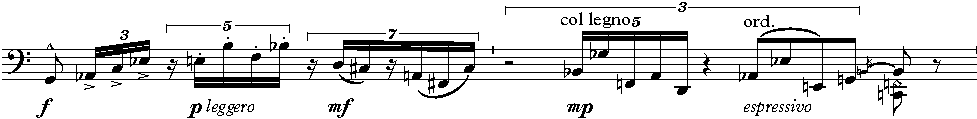
\includegraphics[width=6.5in]{figures/stingray-example.pdf}
        \caption[Self-derivation in Damiani's \emph{Stingray}.]{Self-derivation in Damiani's \emph{Stingray}.}
        \label{fig:stingray}
    \end{figure}
\end{example}

\section{Conclusion}

The algorithms, applications and example presented in this paper represent a major advancement in the study of combination matrices of self-derivation. Arguably the most notable contribution is an algorithm that is simple enough to allow computations by hand, while at the same time fast enough to generate thousands of solutions per second when run by a computer, and general enough to compute solutions for arbitrary problem and row sizes. The ideas in \cite{Starr1984} are invaluable for an understanding and classification of various derivation techniques from a set-theoretic perspective. It also contributes enormously to understanding how a particular class of solutions for the self-derivation problem can be constructed by exploring the permutation cycles of $RT_nI$ operations. What is missing in \cite{Starr1984} is an efficient way to compute combination matrices of self-derivation in a general setting. This shortcoming is addressed in \cite{Kowalski1987b}, which restricts its focus to the self-derivation problem and introduces an efficient algorithm to compute solutions for the 12-tone case. Even though the algorithm devised in \cite{Kowalski1987b} can be generalized to other row sizes, it is not a simple algorith to understand or apply. More importantly, it intentionally avoids computing all possible solutions, sacrificing the less interesting ones for speed. The void that Listing~\ref{allSolutionsRecursive} intends to fill is exactly that of an algorithm that can produce a complete set of solutions given a row and a combination matrix size. The achieved result is straightforward to understand and implement. Devising this algorithm required understanding the problem of self-derivation from from a new point of view, namely that of a structure that can be broken down into three basic constituent parts: a linearized top, a semi-magic square, and an array of derived row transforms. In this formulation, a top, a square and a side are necessary and suficcient to characterize a solution, that is, every solution is uniquely determined by them according to Th.~\ref{topSquareSideTheorem}. Such analysis of the problem paves the way for a much deeper understanding of self-derivation, especially when combined with a simple and fast algorithm capable of unveiling a large amount of solutions within reasonable time. Once the self-derivation problem was broken into parts, each part had to be studied and understood in detail. This study resulted in reducing the body of solutions into equivalence classes under the action of $RTn_I$, the number and size of which depending on retrograde or retrograde inverse-invariance of the row. This body of solutions also groups into classes solutions which are equivalent under permutations of the side vector, leading to Cor~\ref{topSquareSideCorollary}, and further into permutations of repeated semi-magic square rows. Although a significant advance, this paper is still a small toward a more complete understanding of self-derivation, falling short in many aspects. Some of theses aspects will be the subject of the rest of this chapter.

One major weakness of the present implementation is the way tops are pre-computed and stored as binary data. Although this method does improve execution speed, it is impractical, if not impossible, to handle large rows and problem sizes, as the number of possible tops becomes quickly unwieldy. One possibility to mitigate this problem would be to compute tops dinamically, compromising execution speed somewhat. In itself, this workaround would not help with the issue that Listing~\ref{allSolutionsRecursive} can produce an unmanageable amount of solutions, many if not most of them being rather uninteresting compositionally. There is a contradiction between a research goal in the present implementation, which is to devise an algorithm that produces a complete body of solutions, and the compositional goal of utilizing combination matrices to achieve meaningful counterpoint. Modifying the current implementation to focus on more interesting combination matrices is very easy. Besides the choice of row itself, the main contributor to uninteresting solutions is the semi-magic square itself. When 

Output solutions in order
Vectorize vector addition and subtraction
Add parameters to restrict results
Use CUDA and other GPU frameworks
Understand how folding works
Use rotations
Use semi-stochastic matrices for syntax
Understand the algebraic structure and reduce the set of solutions into equivalence classes
